\documentclass[12pt]{article}
\usepackage{trishan2}
\usepackage{parskip}
\usepackage{float}

\title{\textbf{Assignment-5}}
\author{Trishan Mondal, Soumya Dasgupta, Aaratrick Basu}
\date{}

\begin{document}
\maketitle

\section*{Problem \textcolor{maroon}{5.5}}
Let $F(X,Y,Z) = \sum_{i=m}^n F_i(X,Z) Y^{n-i}$. Then for $P = [0:1:0]$
\begin{align*}
   m_P(F) & = m_{\varphi(P)}(F_*)              \\
          & = m_{(0,0)}(\sum_{i=m}^n F_i(X,Z)) \\
          & = m.
\end{align*}

A line $L$ is tangent to $F$ if and only if $I(P, F \cap L) > m_p(F)$, thus we must have
\begin{align*}
   I(P,F \cap L) & = \dim_{k} \mathscr{O}_P(\mathbb{P}^2)/(F_*,L_*)                                                  \\
                 & = \dim_k \mathscr{O}_P(\mathbb{P}^2)/(F(X/Y,1,Z/Y), L/Y)                                          \\
                 & = \dim_k \mathscr{O}_{(0,0)}(\mathbb{A}^2)/(F(X,1,Z), L(X,1,Z)) \mathscr{O}_{(0,0)}(\mathbb{A}^2) \\
                 & = I((0,0), F(X,1,Z) \cap L(X,1,Z)).
\end{align*}
Thus we get that $I((0,0), F(X,1,Z) \cap L(X,1,Z)) > m$, hence $L(X,1,Z)$ is tangent to $F(X,1,Z)$, thus it must be a factor of $F_m(X,Z)$ (by defnition of tangent for an affine curve). Therefore, the tangents to $F$ are determined by the factors of $F_m(X,Z)$.

\section*{Problem \textcolor{maroon}{5.7}}
Let $F$ and $G$ be two plane curves with no common components. Let $L$ be a line not contained in $V(FG) \subseteq \mathbb{P}^2$. Then by problem 12, we know that $F \cap L$ and $G \cap L$ are finite. Now there exists a projective transformation that takes the line $L$ to $Z$. Then under this projective transformation we know that intersection numbers of $F$ and $G$ are preserved. And we have
\begin{align*}
   F \cap G = (\underbrace{(F \cap U) \cap (G \cap U)}_{A}) \cup (\underbrace{(F \cap Z) \cup (G \cap Z)}_{B})
\end{align*}
where $U = \{ [x:y:z] \in \mathbb{P}^2 \mid z = 1 \}$. Note that $B$ is finite by the choice of the line $L$. Now $F \cap U$ and $G \cap U$ are affine curves given by $f = F(X,Y,1)$ and $g = G(X,Y,1)$. Now since $F$ and $G$ does not have any common component so does $f$ and $g$ (since otherwise we would have $hp = f$ and $hq = g$ for some $h,p,q \in k[X,Y]$, then $h^* p^* = F$ and $h^* q^* = G$, but then $h^*$ is a common component of $F$ and $G$, contradiction!). But we have previously shown that if two affine curves have no common component then $f \cap g$ is finite. Hence both $A$ and $B$ are finite, thus $F \cap G$ is finite.

\section*{Problem \textcolor{maroon}{5.12}}
\textbf{Part (a).} Let $P \in [0:1:0] \in F$ where $F$ is a curve of degree of $n$. Let $F(X,Y,Z) = \sum_{i=0}^n F_i(Y,Z)X^i$ with $F_i$ is a form of degree $n-i$ with $F_0 \neq 0$ and let $F_0(Y,Z) = \sum_{i=m}^{m+k} a_i Y^i Z^{n-i}$ (with $m,k \geq 0$ and $m+k \leq n-1$, there is no $Y^n$ term as $P = [0:1:0] \in F$).
\begin{align*}
   \sum_{P \in \mathbb{P}^2} I(P, F \cap X) & = \sum_{P \in F_0 \cap X} I(P, F_0 \cap X)                                                                                                                                                                                    \\
                                            & = \sum_{P \in F_0 \cap X \cap U_1} I(P, F_0 \cap X) + I([0:0:1], F_0 \cap X)                                                                                                                                                  \\
                                            & = \sum_{t \in k} I([0:1:t], F_0 \cap X) + I([0:0:1], F_0 \cap X)                                                                                                                                                              \\
                                            & = \sum_{t \in k} \dim_k \left( \mathscr{O}_{[0:1:t]}(\mathbb{P}^2)/(F_{0*} \cap X_*)\right) + \dim_k \left( \mathscr{O}_{[0:0:1]}(\mathbb{P}^2)/(F_{0*} \cap X_*) \right)                                                     \\
                                            & = \sum_{t \in k} \dim_k\left( \mathscr{O}_{(0,t)}(\mathbb{A}^2)/(F_0(1,Z),X)\mathscr{O}_{(0,t)}(\mathbb{A}^2) \right) + \dim_k \left( \mathscr{O}_{(0,0)}(\mathbb{P}^2)/(F_0(Y,1),X)\mathscr{O}_{(0,0)}(\mathbb{A}^2) \right) \\
                                            & = \sum_{t \in k} I((0,t), F_0(1,Z) \cap X) + \mathrm{ord}_{(0,0)}^X(F_0(Y,1))                                                                                                                                                 \\
                                            & = \sum_{P \in F_0(1,Z) \cap X} I(P, F_0(1,Z) \cap X) + \mathrm{ord}^X_{(0,0)}(F_0(Y,1))                                                                                                                                       \\
                                            & = \deg F_0(1,Z) \deg X + m                                                                                                                                                                                                    \\
                                            & = (n-m) + m = n.
\end{align*}
Hence we have proved that $\sum_{P \in \mathbb{P}^2} I(P, F \cap X) = n$.

\

\noindent\textbf{Part (b).} Now if $L$ is not a line contained in $F$, we can find a projective transformation taking $P \in F \mapsto [0:1:0]$ and $L \mapsto X$, then by part (a), we get that
\begin{align*}
   \sum_{P \in \mathbb{P}^2} I(P, F \cap L) = n.
\end{align*}

\section*{Problem \textcolor{maroon}{5.14}}
We will begin with the assumption, the underlying field $k$ is infinte and algebraically closed (according to contexts). The property of lines passing through points is a projective property. So we can take a suitable projective transformation so that $P_1 = [0:0:1]$. Thus, any line passing through this looks like $ax +by = 0$ where $a,b \in k$. The set of lines passing through $P_1$ is $$A = \qty{x+my : m \in k} \cup \qty{y=0}$$ Since, the field is infinite, there is infinitely many elements in $A$. Given two points in $\mathbb{P}^2$ there is a unique line passing through $P_1$ and that point. Thus the set of lines $$L=\qty{\ell \text{ pass through } P_1 \text{ and }P_{i} : 2 \leq i \leq n} \subset A$$ is finite. So there are only finitely many line in the above set. But in $A$ there are infinitely elements. So, there are infinitely many elements in $A \setminus L$.

\vspace*{0.2cm}

\noindent Since $P_1$ is a simple point of $F$, there is a tangent $T$ at $P$ so that the tangent $T$ don't contained in $V(F)$ (or $F$). From the problem \textcolor{maroon}{5.12} we can say, $$\sum I(P;F\cap T)=n$$ where $n = \deg F$. Thus, If we take $P_2,\cdots,P_m$ be the other intersection points (here $m \leq n$) of $T$ and $F$, by the previous calculation we can say there exists infinitely many lines through $P$ don't intersect $F$ at $P_i$ ($i >1$). These lines are transversal to $F$. $\hfill \blacksquare$

\section*{Problem \textcolor{maroon}{5.18}}

Let us consider the general equation of conic in $\mathbb{P}^2$, that is $$Ax^2+By^2+Cz^2+Exy+Fyz + G zx =0$$ Since the pont $[0:0:1]$ and $[0:1:0]$, $[1:0:0]$ passes through  the above conic we can say, $A=B=C=0$. Thus the equation of conic reduces to $E xy + Fyz+Gzx=0$. Also the points $[1:1:1]$ and $[1:2:3]$ passes through the curve. So we have the following linear equations,
\begin{align*}
   E+F+G                         & =0         \\
   2E+6F +3G                     & =0         \\
   \implies \begin{pmatrix}
               1 & 1 & 1 \\
               2 & 6 & 3
            \end{pmatrix} \begin{pmatrix}
                             E \\ F \\ G
                          \end{pmatrix} & = 0
\end{align*}
Note that the rows of the aboe matrix are linearly independent. So the null space of it must have dimension $1$. Note that $(3, \, -4, \,1)^T$ is a solution to the above matrix equation. Since the dimension of null space is $1$ we can say any other solution must be a scaler multiple of $(3,\, -4, \,1)^T$. So the equation of conic passing through the five  points is $\lambda (3xy -4yz+zx)=0$. This will represent a unique conic in $\mathbb{P}^2$. By contruction the conic is unique! $\hfill \blacksquare$

\section*{Problem \textcolor{maroon}{5.19}}

Let us consider an arbitrary cubic
\begin{align*}
   aX^3 + bX^2Y + cX^2Z + d Y^3 + e XY^2 + f Y^2 Z + g Z^3 + h XZ^2 + i YZ^2 + j XYZ
\end{align*}
Now given that the cubic passes through the following points: $[0 : 0 : 1]$, $[0 : 1 : 1]$, $[1 : 0 : 1]$, $[1 : 1 : 1]$, $[0 : 2 : 1]$, $[2 : 0 : 1]$, $[1 : 2 : 1]$, $[2 : 1 : 1]$, and $[2 : 2 : 1]$ gives us
\begin{align*}
   \begin{pmatrix}
      0 & 0 & 0 & 0 & 0 & 0 & 1 & 0 & 0 & 0 \\
      0 & 0 & 0 & 1 & 0 & 1 & 1 & 0 & 1 & 0 \\
      1 & 0 & 1 & 0 & 0 & 0 & 1 & 1 & 0 & 0 \\
      1 & 1 & 1 & 1 & 1 & 1 & 1 & 1 & 1 & 1 \\
      0 & 0 & 0 & 8 & 0 & 4 & 1 & 0 & 2 & 0 \\
      8 & 0 & 4 & 0 & 0 & 0 & 1 & 2 & 0 & 0 \\
      2 & 2 & 1 & 8 & 4 & 4 & 1 & 1 & 2 & 2 \\
      8 & 4 & 4 & 1 & 2 & 1 & 1 & 2 & 1 & 2 \\
      8 & 8 & 4 & 8 & 8 & 4 & 1 & 2 & 2 & 4
   \end{pmatrix}\begin{pmatrix}
                   a \\ b \\ c \\ d \\ e \\ f \\ g \\ h \\ i \\ j
                \end{pmatrix} = \mathbf{0}.
\end{align*}
The rank of the above matrix is $9$, thus the dimension of the kernel is $1$, hence there exists an unique cubic passing through all the points.

\section*{Problem \textcolor{maroon}{5.25}}

Since the polynomial $F=F_1F_2$ have $c\geq 1$ simple component, the polynomial may not be irreducible. Let, $F=F_1F_2$ and at every point $P$, $m_P(F)= m_P(F_1)+m_P(F_2)$. Thus, \begin{align*}
   \sum_P \frac{m_P(F)(m_P(F)-1)}{2} & = \sum_{P} \frac{(m_P(F_1)+m_P(F_2))(m_P(F_1)+m_P(F_2)-1)}{2}                       \\
                                     & = \sum_{P} \frac{m_P(F_1)(m_P(F_1)-1)}{2} + \sum_{P} \frac{m_P(F_2)(m_P(F_2)-1)}{2} \\&+ \sum_{P}m_P(F_1)m_P(F_2)
\end{align*}
Let, $p = \deg F_1$ and $q = \deg F_2$. If $F_1$ and $F_2$ were irreducible then we must have \begin{align*}
   \sum_P \frac{m_P(F)(m_P(F)-1)}{2}
    & = \sum_{P} \frac{m_P(F_1)(m_P(F_1)-1)}{2} + \sum_{P} \frac{m_P(F_2)(m_P(F_2)-1)}{2}     \\&+ \sum_{P}m_P(F_1)m_P(F_2) \\
    & \overset{\textcolor{maroon}{\ast}}{\leq} \frac{(p-1)(p-2)}{2}+\frac{(q-1)(q-2)}{2} + pq \\
    & = \frac{(p+q-1)(p+q-2)}{2} +1                                                           \\
    & = \frac{(n-1)(n-2)}{2}+1
\end{align*}
here, $\textcolor{maroon}{\ast}$ comes from the \textcolor{maroon}{corollary 1} of B\'ezout's theorem and theorem of section \textcolor{maroon}{5.4}. In this case we had $c=2$. Now we will proceed using induction. Assume the result is true for some curve with $c-1$ simple components. Again assume $F=F1F_2$ with the degrees mentioned above and $F_1$ has $c-1$-simple components and $F_2$ is irreducible. Thus using induction we have,
\begin{align*}
   \sum_P \frac{m_P(F)(m_P(F)-1)}{2}
    & = \sum_{P} \frac{m_P(F_1)(m_P(F_1)-1)}{2} + \sum_{P} \frac{m_P(F_2)(m_P(F_2)-1)}{2}          \\&+ \sum_{P}m_P(F_1)m_P(F_2)\\
    & \leq \underbrace{\frac{(p-1)(p-2)}{2}+c-2}_{\text{induction step}}+\frac{(q-1)(q-2)}{2} + pq \\
    & = \frac{(p+q-1)(p+q-2)}{2} +c-1 = \frac{(n-1)(n-2)}{2}+c-1
\end{align*}
Thus our induction step is complete. It's not hard to note that a polynomial of degree $n$ can have at most $n$ linear factor, i.e atmost $n$ simple components. Thus $c \leq n$ and hence the final term in the above calculation is bounded above by $n(n-1)/2$. $\hfill\blacksquare$

\section*{Problem \textcolor{maroon}{5.28}}

Let \( L \) be a line through \( P \). As \( P = [0,1,0] \), \( L \) must be of the form \( aX+bZ=0 \). If \( b = 0 \), that is, \( L \) is the line \( X = 0 \), then \( L \cap F \) consists of \( [0,1,0] \) and \( [0,0,1] \).
\smallskip

Now suppose that \( b \neq 0 \). Then, any point on \( L \) satisfies \( Z = \frac{-a}{b}X \). Putting this in the polynomial defining \( F \) we get,
\[
   X^{p+1}-Y^p \qty(\frac{-a}{b}) X = X(bX^p+aY^b) = bX (X-\lambda Y)^p,
\]
where \( \lambda^p = \frac{-a}{b} \) and we use the fact that the field is of characteristic \( p \). Hence, either \( X = 0 \) or \( X = \lambda Y \). This gives either \( Z = 0 \) or \( Z = \lambda^{p+1}Y \). So, if \( L \) is not the line \( X = 0 \), \( L \cap F \) consists of the points \( [\lambda y, y, \lambda^{p+1} y], y \in k \), where \( \lambda^p = \frac{-a}{b} \).
\smallskip

We have,
\[
   \pdv{F}{X} = (p+1)X^p = X^p, \quad \pdv{F}{Y} = -pY^{p-1}Z = 0, \quad \pdv{F}{Z} = -Y^p.
\]
Hence, \( [x,y,z] \) is a simple point of \( F \) iff \( x^{p+1} = y^pz \) and one of \( x,y \) is non-zero. The tangent to \( F \) at such a point is then given by \( x^p X -y^p Z = 0 \), which clearly passes through the point \( [0,1,0] \) as required. \(\hfill \blacksquare\)

\section*{Problem \color{maroon}{5.31}}
\textbf{Part (a).} Applying the Pascal's theorem with $P_1 = P_2$, $P_3 = P_4$ and $P_5 = P_6$ we get that, for any triangle $P_1P_3P_5$ inscribed on a cubic, the intersection of the tangent at each vertex with the opposite side of the triangle are collinear. In the given figure $P_1P_3P_5$ is the triangle inscribed on a cubic, and the tangent at $P_1$ intersects the opposite side $P_3P_5$ at $D$, we similarly define $E$ and $F$, then $D,E$ and $F$ are collinear. 
\begin{figure}[H]
   \centering
   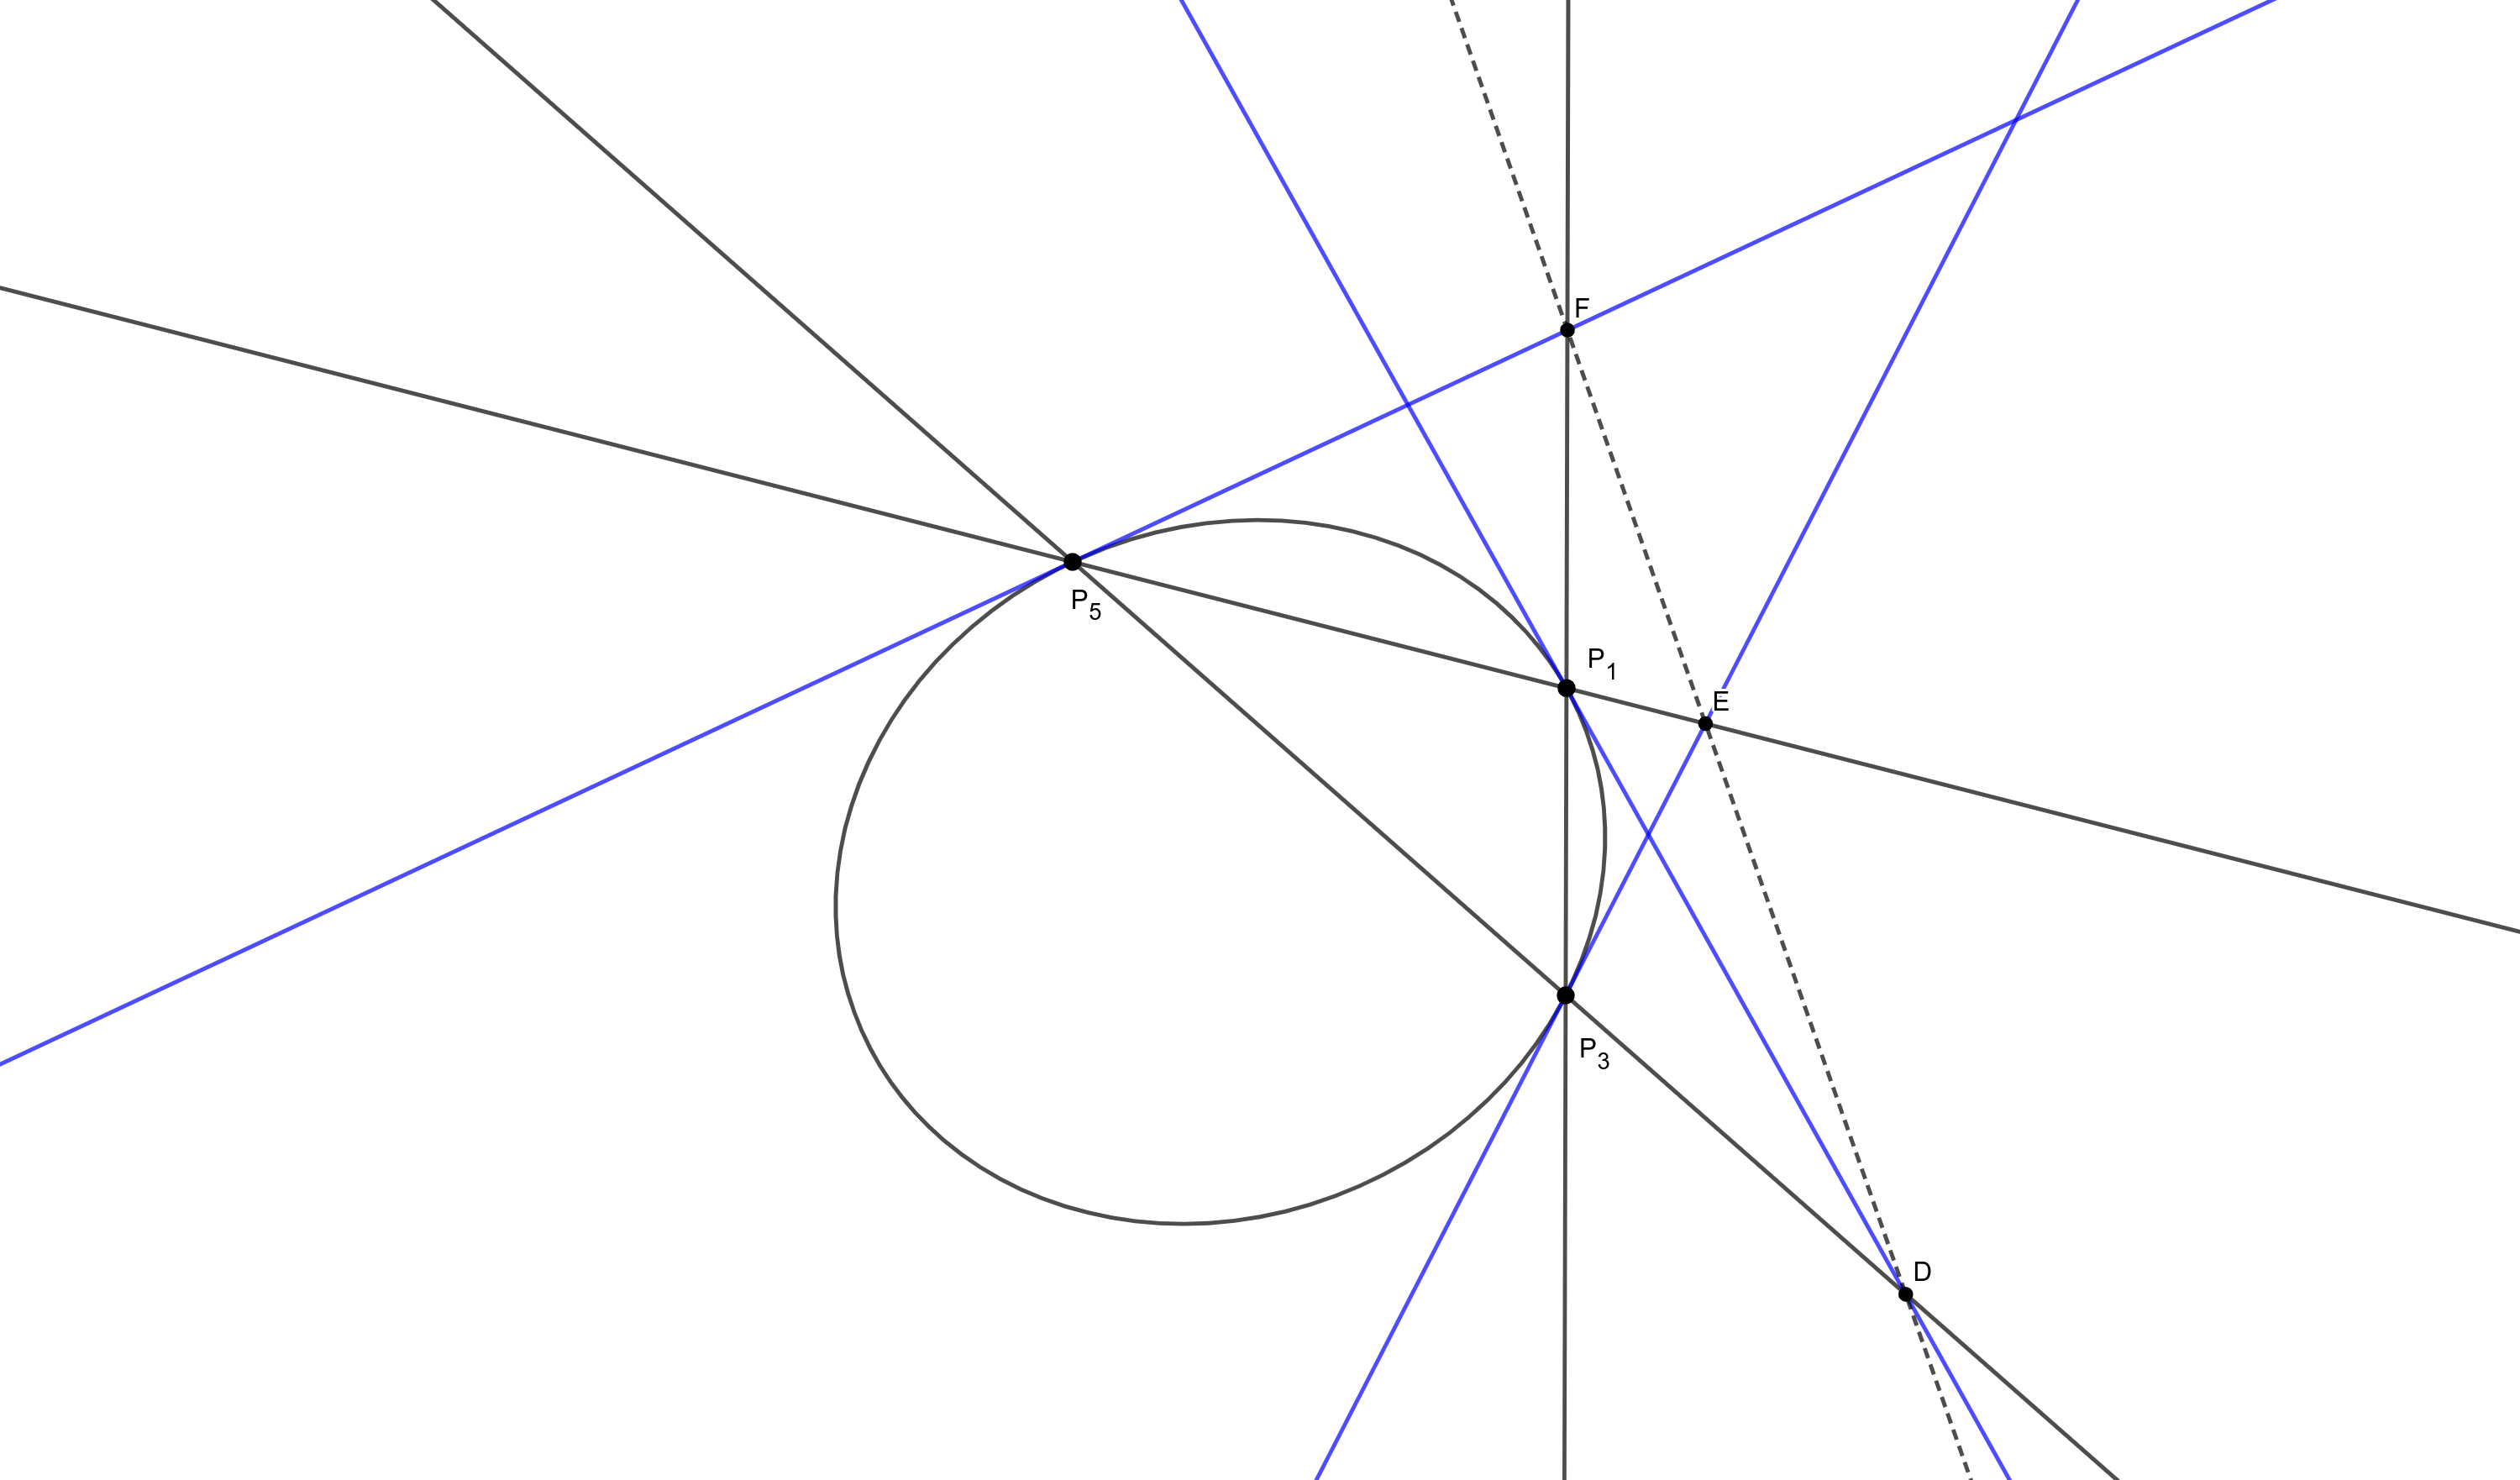
\includegraphics[width=0.8\textwidth]{pascal1.png}
   \caption{Sketch of Pascal's thoerem for $P_1 = P_2$, $P_3 = P_4$ and $P_5 = P_6$.}
\end{figure}

\textbf{Part (b).} Applying the Pascal Theorem with $P_1 = P_2$, we get that for any arbitrary five points $P_1, P_3, P_4, P_5, P_6$ on a cubic, let $E = P_1 P_3 \cap P_5 P_6$ and $F = P_1 P_6 \cap P_3 P_4$ and let $D = EF \cap P_4 P_5$, then $DA$ is the tangent at $A$ to the given cubic. 
\begin{figure}[H]
   \centering
   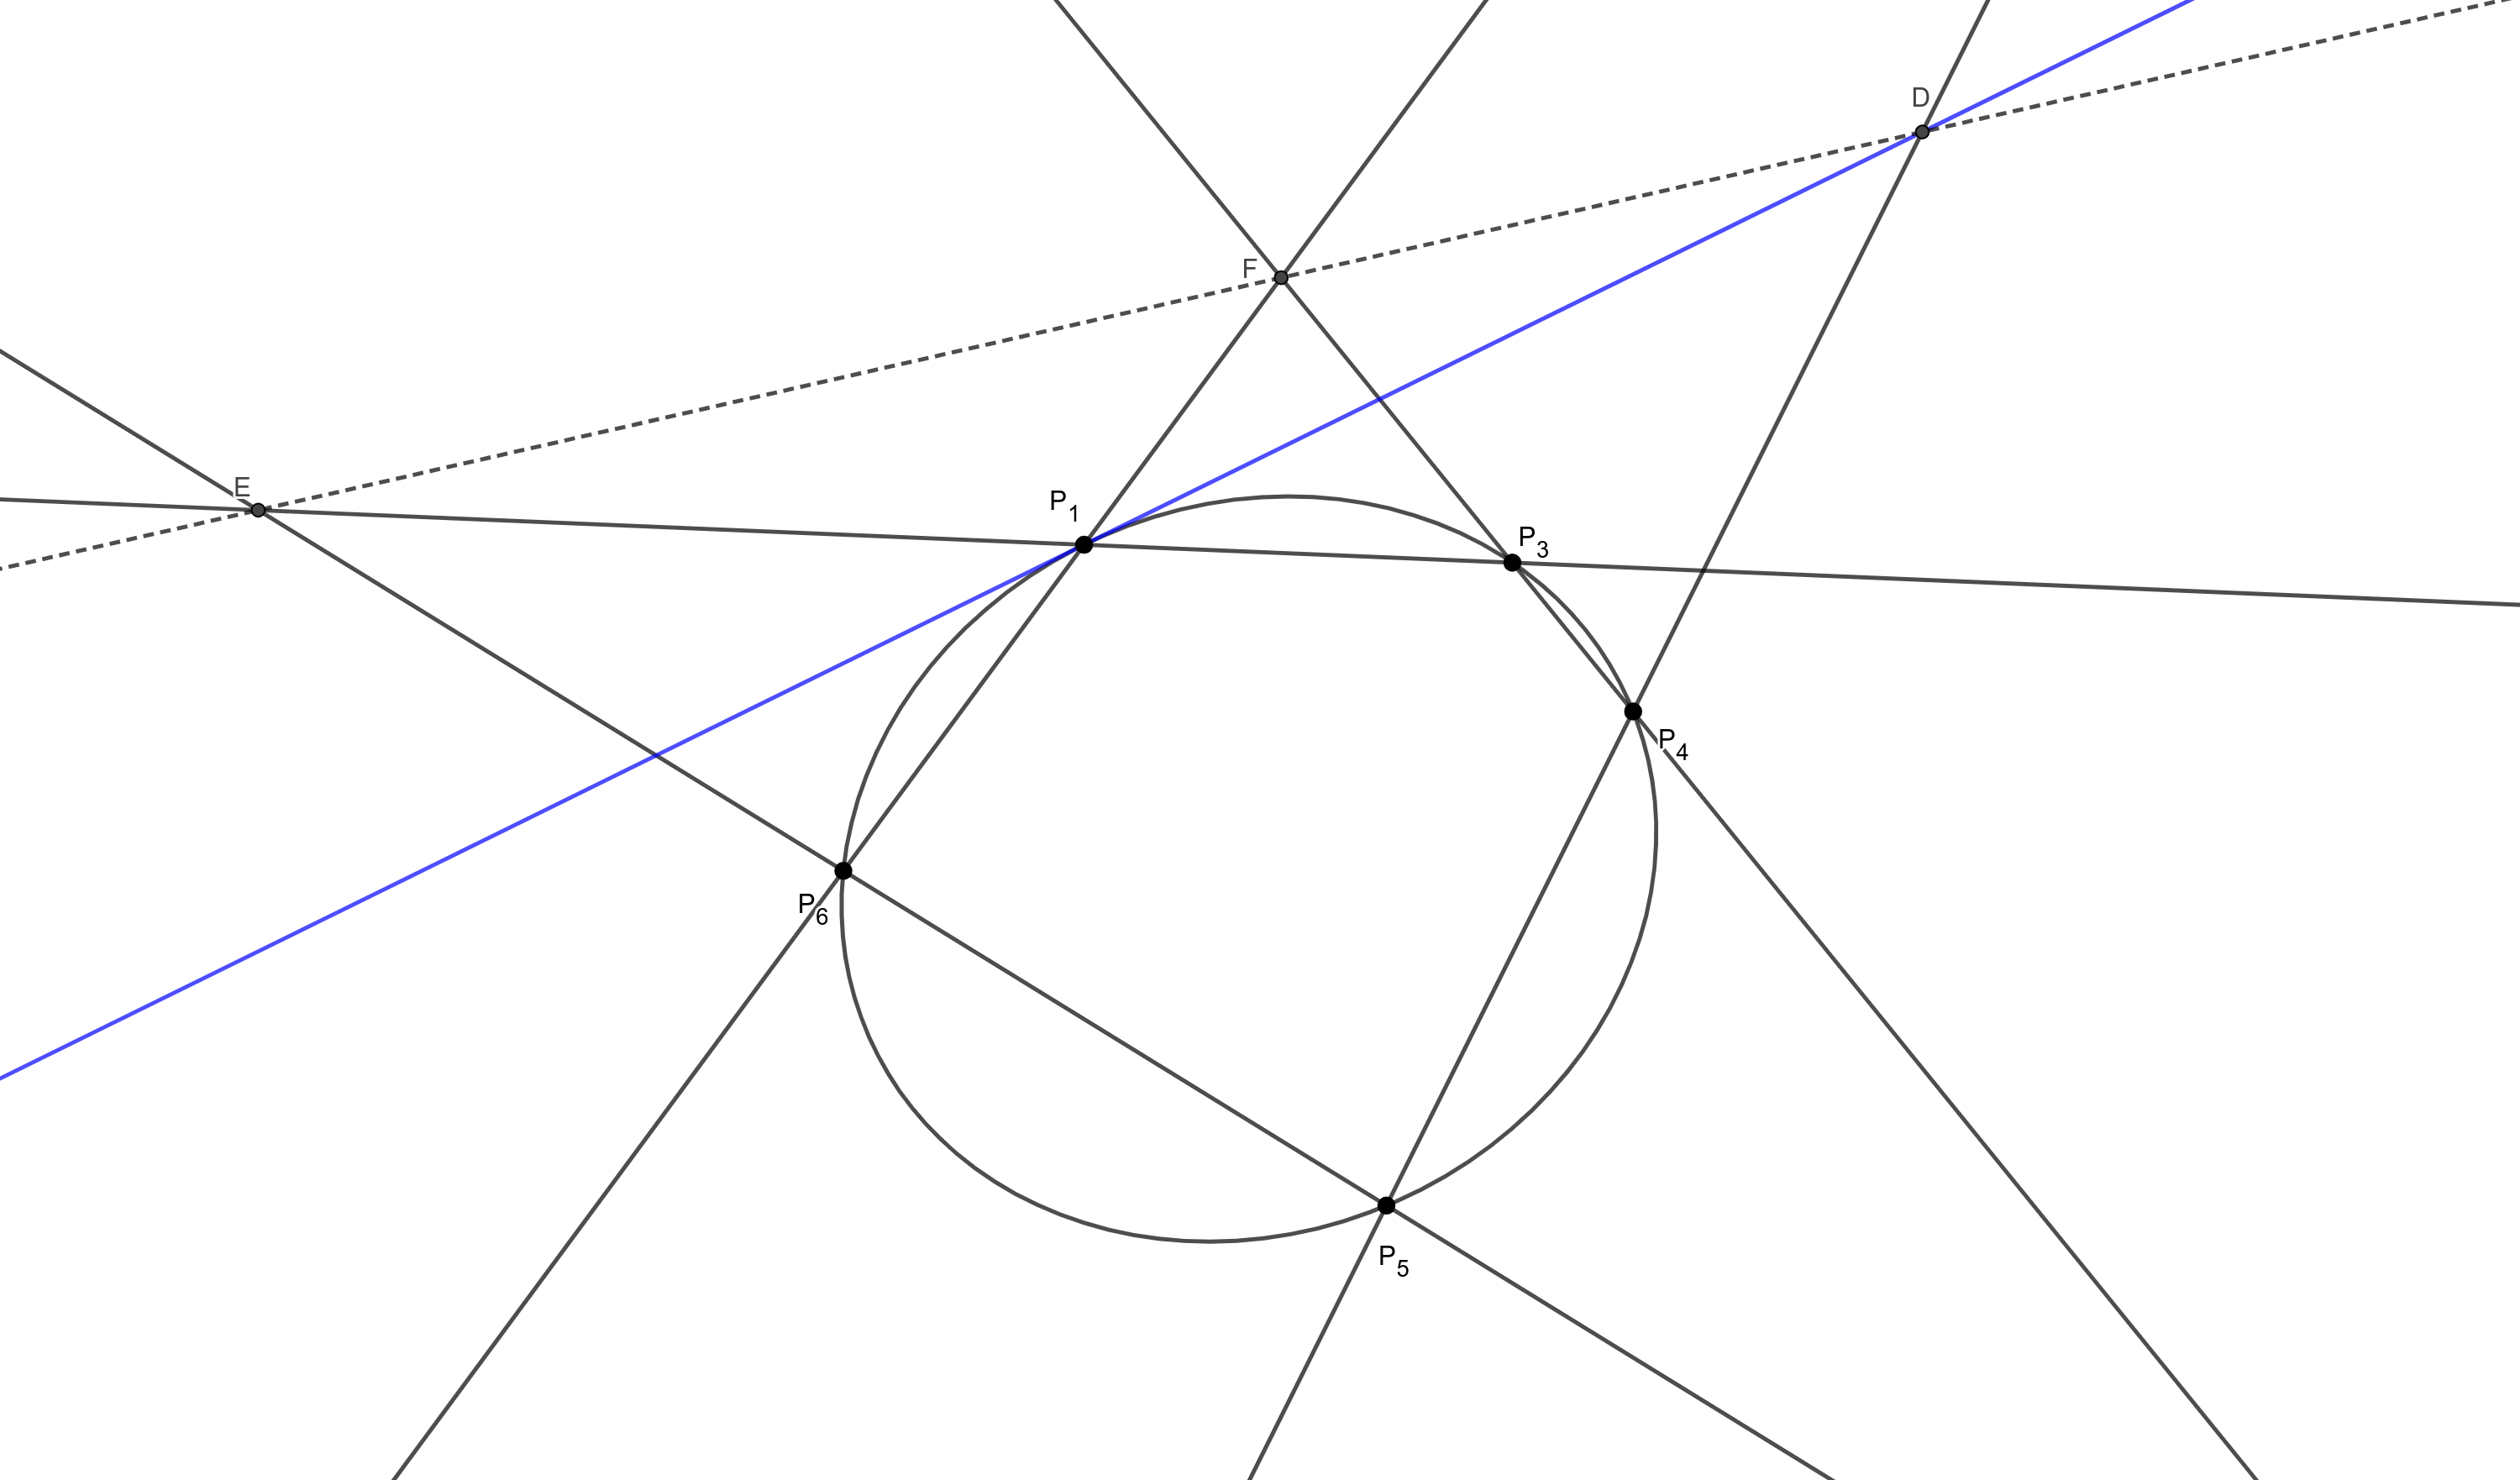
\includegraphics[width=0.8\textwidth]{pascal2.png}
   \caption{Sketch of Pascal's thoerem for $P_1 = P_2$.}
\end{figure}

\textbf{Part (c).} Using part (b), given any point $P$ and a conic $\mathcal{C}$, we can construct a tangent at $P$ to $\mathcal{C}$, as follows: let $P_1, \dots, P_4$ be four distinct points on the conic $\mathcal{C}$. Now let $E = PP_1 \cap P_3P_4$ and $F = PP_4 \cap P_1 P_2$ and let $D = EF \cap P_2P_3$, then $DP$ is the tangent at $P$ to $\mathcal{C}$. Thus we can construct the tangent on a cubic, using only a straight-edge.


\end{document}